\section{Extraction de l'information}
L'extraction se compose des phases de segmentation du texte, de la reconnaissance des entités nommées (REN), de l'analyse des relations entre entités. Toutes les étapes qui extraient, d'une manière ou d'une autre, de l'information depuis le document source ou d'un fragment de celui-ci. 
La finalité des opérations d'extraction de l'information dans le cadre de ce processus est de fournir un tableau de données, ou un système de table de données, reprenant toutes les informations semi-structurées du document source mises sous forme structurée, de sorte que ces données puissent directement servir à des études quantitatives.

\subsection{Segmentation du texte}
La segmentation du texte est l'une des premières phases du processus. Comme préalablement expliqué, les rentes sont ordonnées dans le registre en fonction d'éléments topographiques (escroete, connétablie, rang de voie) et chacun de ces éléments topographiques est renseigné par un marqueur de structure. Deux précisions  importantes : premièrement, les éléments topographiques représentés par ces marqueurs sont hiérarchisés; secondement, chacun de ces marqueurs de structure est unique\footnote{A l'exception des marqueurs de rang de voie.}.
Cela signifie, d'une part, que les rentes sont toujours situées dans une connétablie, elle-même située au sein d'une escroete et d’autre part, qu'une rente ne peut appartenir qu'à une et une seule connétablie, au même titre qu'une connétablie ne peut appartenir qu'à une et une seule escroete.
Le cas des indications du rang de voie est plus particulier dans le sens où selon la nature de la connétablie - qui n'est pas dans tous les cas, une rue ayant deux rangées de propriétés bâties - elle peut ne pas être présente et aussi parce que les rangs de voie, à la différence des autres éléments topographiques, ne disposent pas d'identification unique.
Les marqueurs des structures, étant chacun unique, ils constituent des clés idéales pour identifier une rente ou un groupement de rentes en fonction d'un élément topographique. 

C'est donc sur base de la reconnaissance de ces marqueurs par des \textit{regex}\footnote{appelées aussi \og expressions régulières\fg{}.} que l'algorithme va, de manière récursive, découper le texte initial en plusieurs parties. Dans un même temps, l'algorithme va construire un tableau de données afin de  recueillir les informations. 

La figure \ref{schemaSeg} illustre par un organigramme les étapes effectuées par le script de segmentation du texte source.
L’algorithme va en premier lieu parcourir le fichier et indexer tous les marqueurs d'escroete. Pour chaque marqueur d'escroete indexé, la section concernant celle-ci, ainsi que la définition correspondante, va être capturée et stockée dans un tableau de données\footnote{appelé aussi \textit{dataframe}, ou \textit{df} en abrégé}. Maintenant que le document texte est découpé au niveau des marqueurs d'escroete, pour chaque escroete répertoriée dans le tableau de données, une fonction similaire est appelée  en prenant comme argument la section de l'escroete concernée au lieu du texte source.
La fonction appelée détecte et indexe les marqueurs de connétablie. 
Ensuite pour chaque marqueur de connétablie indexé, la section est capturée et stockée dans un nouveau tableau de données, où pour chacune des connétablies, à nouveau, une fonction similaire est appelée pour exécuter les mêmes opérations ( indexation des marqueurs, capture et stockage des sections ) au niveau des rangs de voie, puis encore une fois au niveau des rentes.
Lorsque les sections de toutes les rentes d'un rang de voie sont stockées dans un tableau de données avec leur clé
\footnote{La clé prend la valeur du marqueur, dans le cas des rentes il s'agit du numéro de rente}, 
la fonction appelée renvoie ce tableau à la fonction appelante, c’est-à-dire à la fonction d'extraction des rangs de voie, si la connétablie en possède, sinon la fonction d'extraction des connétablies dans l'autre cas. La fonction appelante va collecter tous les tableaux - un pour chacune des sections qu'elle stocke dans son propre tableau de données - et va ensuite les fusionner en y rajoutant sa propre clé (indicateur du rang de voie ou numéro de connétablie). L'opération est répétée ensuite vers les fonctions appelantes supérieures.

De l'exécution du script résulte un tableau de données contenant la clé et la définition de chaque escroete, de chaque connétablie, et de chaque rente. La création d'un système de tables de données au lieu d'un grand tableau de données a également été envisagée, cependant la solution du tableau de données a été retenue pour sa plus grande simplicité de mise en place et d'utilisation pour et parce qu'elle était suffisante pour les besoins du projet. L'alternative du système de table de données sera abordée avec plus de précision  dans la partie \textit{Discussion} du mémoire.

\begin{figure}[ht] % insère une figure ici (h = "here")
    \centering
    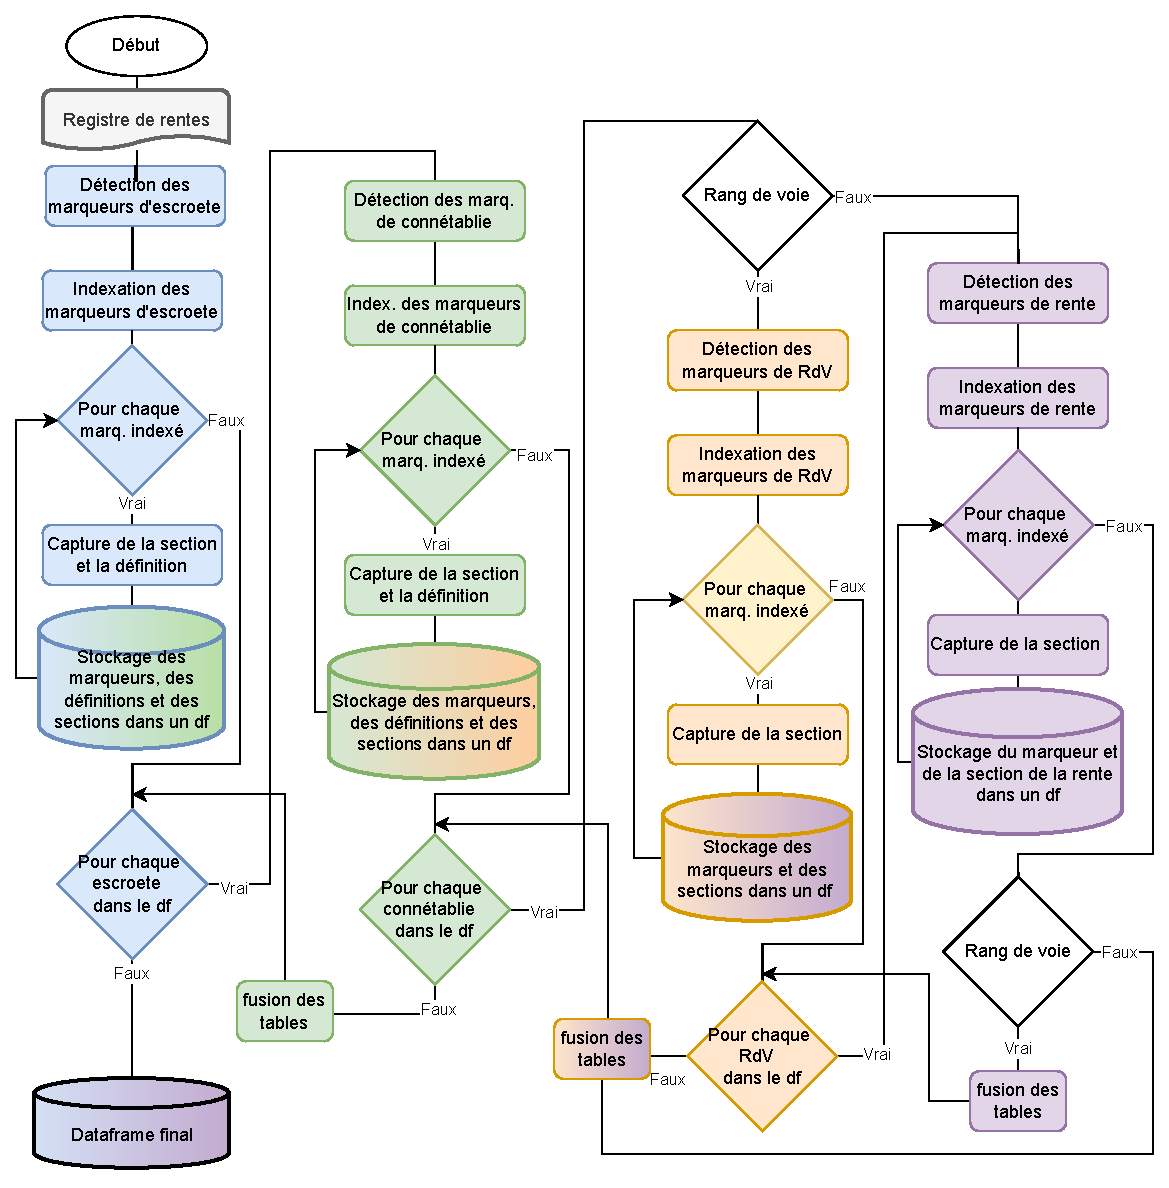
\includegraphics[scale=0.75]{2.Methods/Img/seg.drawio.pdf} 
    \caption{Organigramme de la segmentation automatisée du registre de rente.}
    \label{schemaSeg}
\end{figure}

\subsection{Reconnaissance et extraction des entités nommées}
Le concept d'\textit{entité nommée} désigne les unités textuelles possédant une fonction de référentiel au sein d'un contexte. Les noms propres, de personnes, de lieux, ou d'organisations, en sont l'exemple le plus évident, mais les entités nommées peuvent prendre bien d'autres formes telles que des pronoms, des valeurs numériques ou des descriptions définies \parencite{omrane_les_2010,nadeau_survey_2007}.

Selon le type d'entité nommée que l'on cherche à détecter et la nature du texte, la reconnaissance d'entités nommées peut s'avérer être une tâche complexe. Dans le cas de nos travaux, la reconnaissance d'entité se limite à la détection d'anthroponymes et de lieux (dit \textit{toponyme}) et ne s'avère par conséquent relativement pas trop complexe. Cependant, au vu des ressources possédées, ni les approches \textit{orientées connaissances}, utilisant des lexiques, ni les approches \textit{orientées données}, basées sur un apprentissage automatique,  ne sont exploitables. Il faut donc retourner à une  approche plus historique qui se concentre sur la reconnaissance de caractères morphologiques tels que les majuscules \parencite{nouvel_reconnaissance_2012}. 

La méthode utilisée se base intégralement sur les travaux de S. De Valeriola. Celle-ci conçoit les anthroponymes comme l'assemblage d'un  nom de baptême et d' un patronyme. Patronyme qui est constitué d'un ensemble d'unités textuelles  pouvant être rassemblées en  groupes de mots ayant la même structure. Plus concrètement, on retrouve, potentiellement,  une ou plusieurs particules  suivies d'un ou plusieurs \og noms \fg{}. La méthode combine donc trois expressions régulières afin de détecter ces trois éléments évoqués : le prénom, la ou les éventuelles particules liées au nom de famille et le ou les noms \parencite{de_valeriola_lordinateur_2021}. L'approche développée est évidemment spécifique aux anthroponymes du contexte historique décrit dans la partie \textit{Introduction}.

\subsection{Analyse des relations entre entités}
Rappelons, que dans ce contexte, les entités nommées sont presque uniquement des anthroponymes, et à de rares occasions, un lieu comme une porte d'enceinte ou une place de marché, et que les relations qui les unissent sont des liens de mitoyenneté.
L'analyse des relations entre entités nommées se fait une fois de plus à l'aide d'expression régulière. Les entrées du registre de rentes, si en tant que telles, sont des données textuelles non structurées, présentent néanmoins un certain formalisme dans leur construction. G. Espinas nous dit à ce propos : 
\begin{displayquote}
    \og Les énoncés des propriétés et de revenus se présentent selon des conditions et même dans des formes tout à fait analogues, à peu près identiques, qui peuvent se schématiser ainsi : « Sur la ou sur les maisons d’un tel et sur tout le tenement — ki fu a un tel, au besoin — , qui siet entre le tenement d’un tel et le tenement d’un tel — , ki, de part et d’autre, furent à un tel, au besoin — , dou fons de le terre, ou apries le fons de le terre, régulièrement, ou sans indication d’affectation par exception — , tant de rente de telle nature, d’un seul ou de plusieurs éléments ».\fg{}
    \footfullcite[p.113]{espinas_les_1933}
\end{displayquote} 
\vspace{0,5cm}
Pour extraire les entités nommées et définir leurs relations, nous pouvons segmenter le texte de la rente en deux parties, de part et d'autre de l'expression \og \textit{qui siet entre} \fg{}. Nous récupérons ainsi, dans la première partie, le nom du débiteur, et dans la seconde partie, les noms de ceux avec qui le débiteur partage un lien de mitoyenneté.




